\documentclass[xcolor=x11names,compress]{beamer}

\usetheme[pageofpages=of,
          alternativetitlepage=true,
          %titlepagelogo=./imgs/uni_sbg_logo_sw.JPG,
		  ]{Mp}
\usepackage[american,austrian]{babel}  % language support
\usepackage{graphicx}
\usepackage{listings}
\usepackage{color}
\usepackage{color}

\definecolor{verylightgrey}{HTML}{EEEEEE}
\definecolor{lightgrey}{HTML}{DDDDDD}
\definecolor{darkgrey}{HTML}{999999}
\definecolor{blue}{HTML}{009EE0}
\definecolor{green}{HTML}{97BE0D}
\definecolor{orange}{HTML}{F29400}

\lstdefinelanguage{JavaScript}{
	keywords={
				break, case, catch, continue, debugger, default, delete, do, else, 
				finally, for, function, if, in, instanceof, new, return, switch, 
				this, throw, try, typeof, var, void, while, with
				},
	keywordstyle=\color{blue!70!black}\ttfamily,
	ndkeywords={class, export, boolean, throw, implements, import, this},
	ndkeywordstyle=\color{green!70!black}\ttfamily,
	identifierstyle=\color{black}\ttfamily,
	stringstyle=\color{orange}\ttfamily,
	sensitive=false,
	comment=[l]{//},
	morecomment=[s]{/*}{*/},
	commentstyle=\color{darkgrey}\itshape,
	stringstyle=\color{orange!90!black}\ttfamily,
	morestring=[b]',
	morestring=[b]",
	belowcaptionskip=1\baselineskip,
	breaklines=false,
	extendedchars=true,
	frame=none,
	frameround=tttt,	% or values t or f
	backgroundcolor=\color{white},
	showstringspaces=false,
	showspaces=false,
	showtabs=true,
	captionpos=b,
	numbers=left,
    numberstyle=\footnotesize,
    numbersep=9pt,
    tabsize=2,
}

\title{ACDC4JS}
\subtitle{How to analyze a JavaScript garbage collector}
\author{Mario Preishuber}
\institute[2013]{University of Salzburg}

\begin{document}
	
	\begin{frame}
		\titlepage
	\end{frame}

	\begin{frame}
		\frametitle{Content}
		\setcounter{tocdepth}{1}
		\tableofcontents
	\end{frame}
	
	%-----------------------------------------------------------------------
	% INTRODUCTION SECTION
	%-----------------------------------------------------------------------
	
	\section{Introduction}	
	\begin{frame}
		\frametitle{Introduction}
		ACDC: Towards a Universal Mutator for
		Benchmarking Heap Management Systems \\
		\bigskip
		\textbf{Authors} \\
		Martin Aigner \\ 
		Christoph M. Kirsch \\
		\bigskip
		\textit{ACDC is an open-source benchmark that be configured to emulate explicit single- and multithreaded mutator behavior 
		for measuring allocation, deallocation, and memory access throughput as well as memory consumption and multicore 
		scalability of an allocator.}
		
	\end{frame}
	
	\subsection{Memory management}
	\begin{frame}
		\frametitle{Memory management}
		\begin{columns}
			\begin{column}{.1\linewidth}
				\includegraphics<1>[width=5.5em]{./imgs/memory_0.pdf}
				\includegraphics<2>[width=5.5em]{./imgs/memory_1.pdf}
				\includegraphics<3>[width=5.5em]{./imgs/memory_2.pdf}
				\includegraphics<4>[width=5.5em]{./imgs/memory_3.pdf}
				\includegraphics<5>[width=5.5em]{./imgs/memory_4.pdf}
				\includegraphics<6>[width=5.5em]{./imgs/memory_5.pdf}
				\includegraphics<7>[width=5.5em]{./imgs/memory_6.pdf}
				\includegraphics<8>[width=5.5em]{./imgs/memory_6.pdf}
				\includegraphics<9>[width=5.5em]{./imgs/memory_6.pdf}
			\end{column}
			\begin{column}{.7\linewidth}
				\begin{itemize}
					\item Typical memory structure
					\begin{enumerate}
						\item Program code
						\item Constants (e.g. strings) 
						\item Heap
						\item Stack
					\end{enumerate}
				
					\pause
					\pause
					\pause
					\pause
					\pause
					\pause
					\pause
					
					\item Memory management in C
					\begin{itemize}
						\item \textbf{Allocation} \texttt{malloc()}
						\item \textbf{Deallocation} \texttt{free()}
					\end{itemize}
		
					\pause
		
					\item Memory management in JavaScript
					\begin{itemize}	
						\item \textbf{Allocation} automatically by initialization 
						\item \textbf{Deallocation} automatically done by the garbage collector (GC)
					\end{itemize}
				\end{itemize}
			\end{column}
		\end{columns}
	\end{frame}
	
	\begin{frame}[fragile]
		\frametitle{Memory management}
			\begin{lstlisting}[language=JavaScript]
				// C: allocates and deallocate memory for a string
				char *s = malloc(4*sizeof(char));
				strncpy(s, "abc\0", 4);
				...
				free(s);
			\end{lstlisting}			
			
			\pause
			
			\begin{lstlisting}[language=JavaScript]
				// JS: allocates and deallocate memory for a string
				var s = "abc";
				...
				dosomething(s);		// last access
			\end{lstlisting}	
			
	\end{frame}
	
	\subsection{Garbage Collector} 
	\begin{frame}
		\frametitle{Garbage Collector}
		\newtheorem{general problem}{General problem}
		\begin{general problem}[] \label{gp:garbage_collector}
			automatically finding whether some memory is not needed anymore
		\end{general problem}
		
		\begin{itemize}
			\item Embedded piece of software
			\item Track memory allocation
			\item Automatically free  
			\item This process is an approximation
			\item The general problem is undecidable
			\begin{itemize}
				\item decision problem for which it is impossible to construct a single algorithm that always leads to a correct yes-or-no answer
			\end{itemize}
		\end{itemize}
	\end{frame}
	
	%-----------------------------------------------------------------------
	% PROBLEM DEFINITION SECTION
	%-----------------------------------------------------------------------
	\section{Problem Definition} 
	\begin{frame}
		\frametitle{Problem Definition}
		The purpose of ACDC4JS is to analyze the efficiency of the garbage collector in JavaScript virtual machines, especially Google's V8.
	\end{frame}
	
	%-----------------------------------------------------------------------
	% SOLUTION SECTION
	%-----------------------------------------------------------------------
	\section{Solution}

	\begin{frame}
		\frametitle{Content}
		\setcounter{tocdepth}{2}
		\tableofcontents[currentsection]
	\end{frame}

	\subsection{Step 1: Get some data}
	\begin{frame}
		\frametitle{Step 1: Get some data}
		\begin{itemize}
			\item Get informations about the garbage collector (whitebox)
			\begin{itemize}
				\item collection cycle
				\item quantity of collected memory
				\item number of collected objects
				\item type of garbage collection
			\end{itemize}
			
			\pause
			
			\item Prepare a simple mutator (blackbox)
			\begin{itemize}
				\item Number of allocated objects
				\item Number of live objects
				\item Size of an object
			\end{itemize}
			
			\pause
			
			\item Wrap system measurements (blackbox)
			\begin{itemize}
				\item Execution time
				\item Real memory (resident set size) 
			\end{itemize}
		\end{itemize}
	\end{frame}
	
	\subsection{Step 2: Compare data}
	\begin{frame}
		\frametitle{Step 2: Compare data}
		Compare as much as possible of the collected data with an other JavaScript engine.
		\begin{itemize}
			\item V8 (Google Chrome) vs. Spidermonkey (Mozilla Firefox)
		\end{itemize} 
		%\center{ 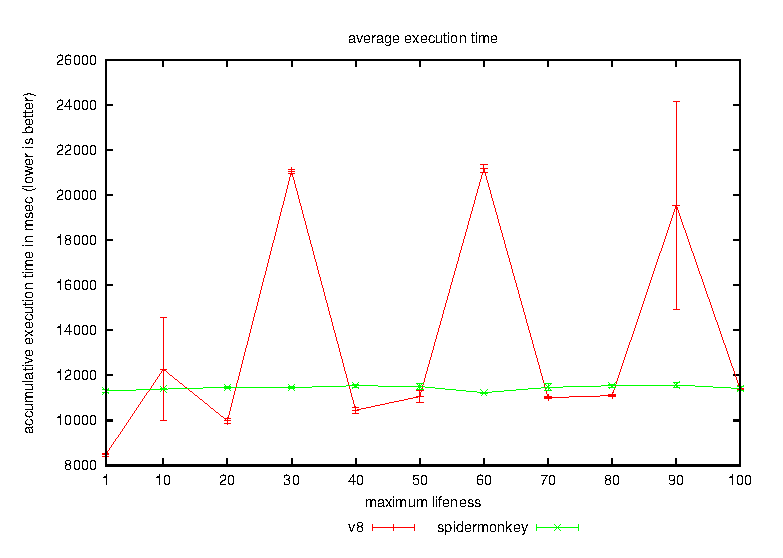
\includegraphics[width=18em]{./imgs/acdc_multi_exec_time.eps} }
	\end{frame}
	
	\subsection{Step 3: Heap model}
	\begin{frame}
		\frametitle{Step 3: Heap model}
		\begin{itemize}
			\item Important for mutator implementation
			\item Customizations
			\begin{itemize}
				\item Custom Chromium binary
				\item Custom V8 binary
			\end{itemize}
			
			\pause
			
			\item Tools for JavaScript heap analyzation
			\begin{itemize}
				\item AutomatedUserInteraction
				\item HeapSnapshotAnalyzer
			\end{itemize}
		\end{itemize}
	\end{frame}

	\subsubsection{Step 3: Heap model}
	\begin{frame}
		\frametitle{Step 3: Heap model}		
		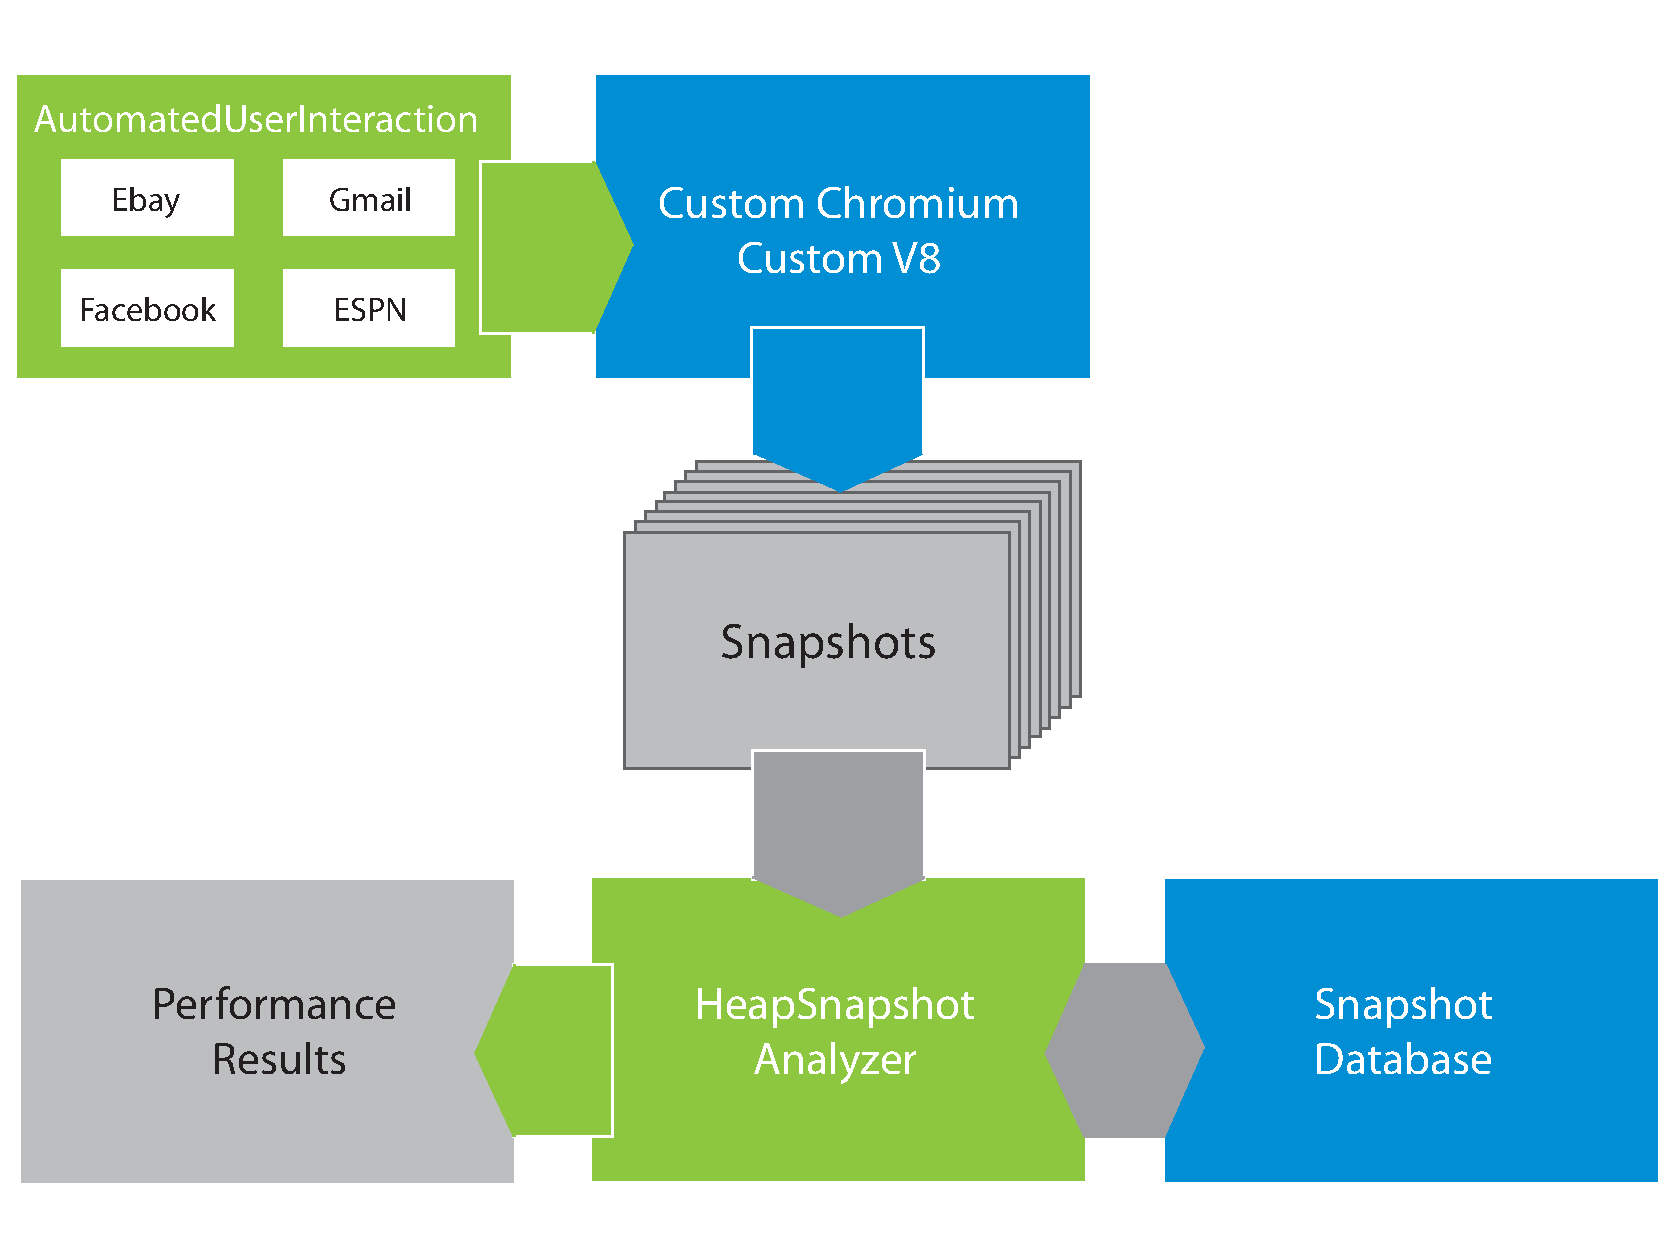
\includegraphics[width=26em]{./imgs/solution_h.pdf}
	\end{frame}

	\subsubsection{Customizations}
	\begin{frame}
		\frametitle{Customizations}
		\begin{columns}
			\begin{column}{.55\linewidth}
				Custom Chromium binary
				\begin{itemize}
					\item Used flags
					\begin{itemize}
						\item \texttt{no\_sandbox} 						% Disables the sandbox for all process types that are normally sandboxed.
					\end{itemize}
				\end{itemize}
			
				Custom V8 binary
				\begin{itemize}
					\item New flags
					\begin{itemize}
						\item \texttt{automatic\_heap\_snapshots} 		% create heap snapshot automatically every heap-snapshot-interval KBs
						\item \texttt{heap\_snapshot\_interval} 		% heap snapshot interval in KB
						\item \texttt{heap\_snapshot\_prefix} 			% prefix for the .heapsnapshot files
					\end{itemize}
					\item Used flags
					\begin{itemize}
						\item \texttt{gc\_interval} 					% garbage collect after n allocations
					\end{itemize}
				\end{itemize}
			\end{column}
			\begin{column}{.35\linewidth}			
				\includegraphics<1>[width=9em]{./imgs/chromium_v.pdf}
			\end{column}
		\end{columns}
	\end{frame}

	\subsubsection{AutomatedUserInteraction}
	\begin{frame}
		\frametitle{AutomatedUserInteraction}
		\begin{itemize}
			\item Java application
			\item SeleniumHQ framework for automated user interaction
			\begin{itemize}
				\item \href{http://www.seleniumhq.org/}{http://www.seleniumhq.org}
			\end{itemize}
			\item Web applications
			\begin{itemize}
				\item \textbf{News:} CNN, ESPN, The Economist
				\item \textbf{Email:} Gmail, Hotmail
				\item \textbf{Shops:} Ebay, Amazon
				\item \textbf{Maps:} Google, Bing
				\item \textbf{Search:} Google, Bing
				\item \textbf{Social:} Facebook, Google Plus
			\end{itemize}
		\end{itemize}
	\end{frame}
	
	\subsubsection{HeapSnapshotAnalyzer}
	\begin{frame}
		\frametitle{HeapSnapshotAnalyzer}
		\begin{itemize}
			\item Java application
			\item PostgreSQL 9.3
			\item Write snapshots into DB
			
			\pause
			
			\item Analyzation of the heap graph
			\begin{itemize}
				 \item Number of leafs
				 \item Number of nodes
				 \item Number of edges
				 \item Number of strongly connected components
			\end{itemize}
			
			\pause 
			
			\item Node characteristics
			\begin{itemize} 
				 \item In-degree
				 \item Out-degree
				 \item Root distance
				 \item Node size 
			\end{itemize}
		\end{itemize} 
	\end{frame}
	
	\subsection{Step 4: JavaScript mutator}
	\begin{frame}
		\frametitle{Step 4: JavaScript mutator}
%		Develop a universal JavaScript mutator based on the real web application analyzation results.  
		Develop a 
		\begin{itemize}
			\item Universal JavaScript mutator
			\item Based on the original ACDC implementation.
		\end{itemize}
		
		\pause
		
		Extend this mutator
		\begin{itemize}
			\item With special features for garbage collector measurements
			\item Based on the analysis results simulate
			\begin{itemize}
				\item real web applications and
				\item corner cases. 
			\end{itemize}
		\end{itemize}
	\end{frame}
	
	%-----------------------------------------------------------------------
	% CONCLUSION SECTION
	%-----------------------------------------------------------------------
	\section{Conclusion}
	\begin{frame}
		\frametitle{Conclusion}
		Done so far:
		\begin{itemize}
			\item Analyzed garbage collector behavior
			\item Analyzed real web application heap behavior
		\end{itemize}
		To do:
		\begin{itemize}
			\item Complete the implementation of the mutator
		\end{itemize}
	\end{frame}
	
	%-----------------------------------------------------------------------
	% QUESTIONS SECTION
	%-----------------------------------------------------------------------
	\section{Questions}
	\begin{frame}
		\frametitle{Thank you for your attention!}
		\center { \Large{Questions?} }
	\end{frame}
	
\end{document}